

\chapter{High Valence Vertices}\label{ch:high_valence}

High valence vertices are a mesh feature which cause significant degredation in
DAGMC ray tracing performance. The valence of a vertex in a mesh is defined as
the number of edges connected to that vertex. \textit{High} valence vertices are
defined as vertices connected to an unusually large number of edges. This
region, known as a high valence region, will typically take on a fan-like shape
as seen in Figure \ref{fig:hv_examples}.  The geometric origins of high valence
regions are typically a planar surface intersected with some form of curved
boundary condition. 

\begin{figure}[H]
  \centering
  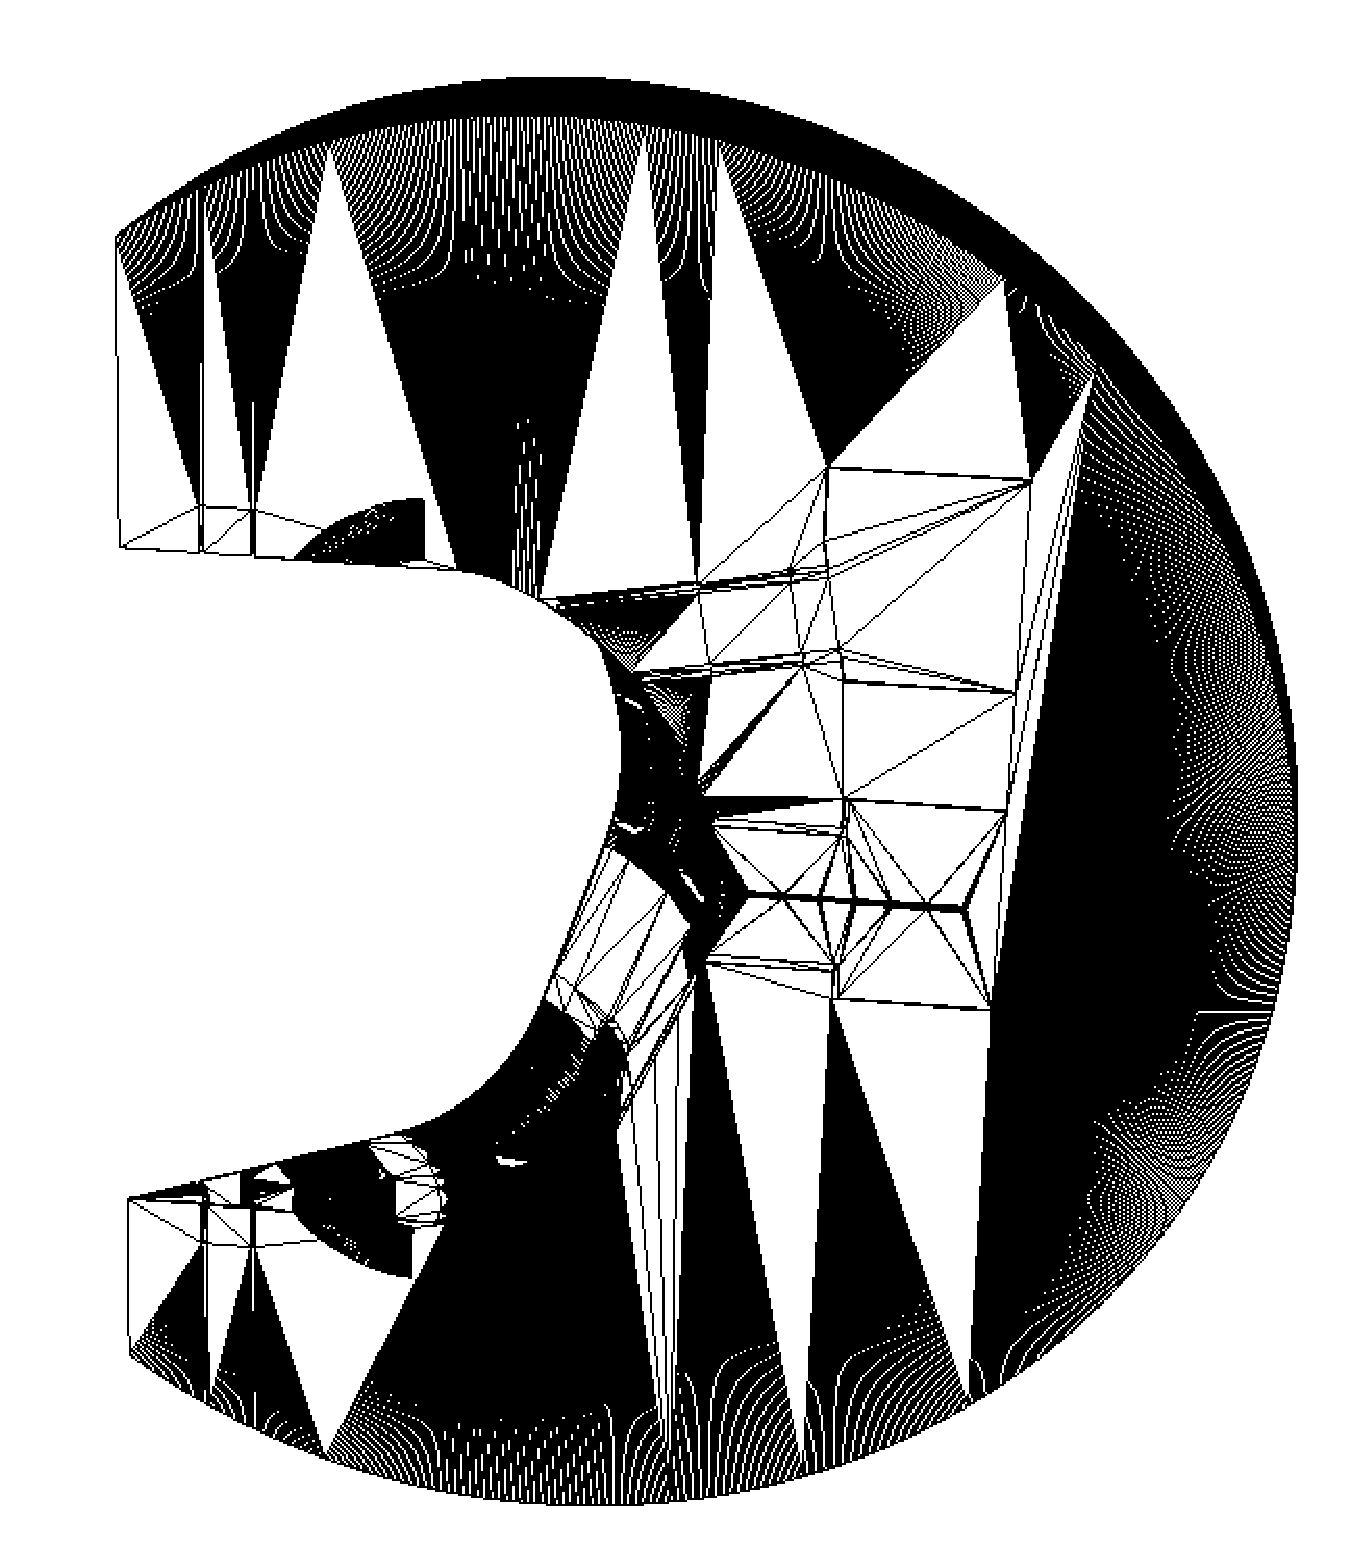
\includegraphics[scale=0.2]{iter_sideon.eps}
  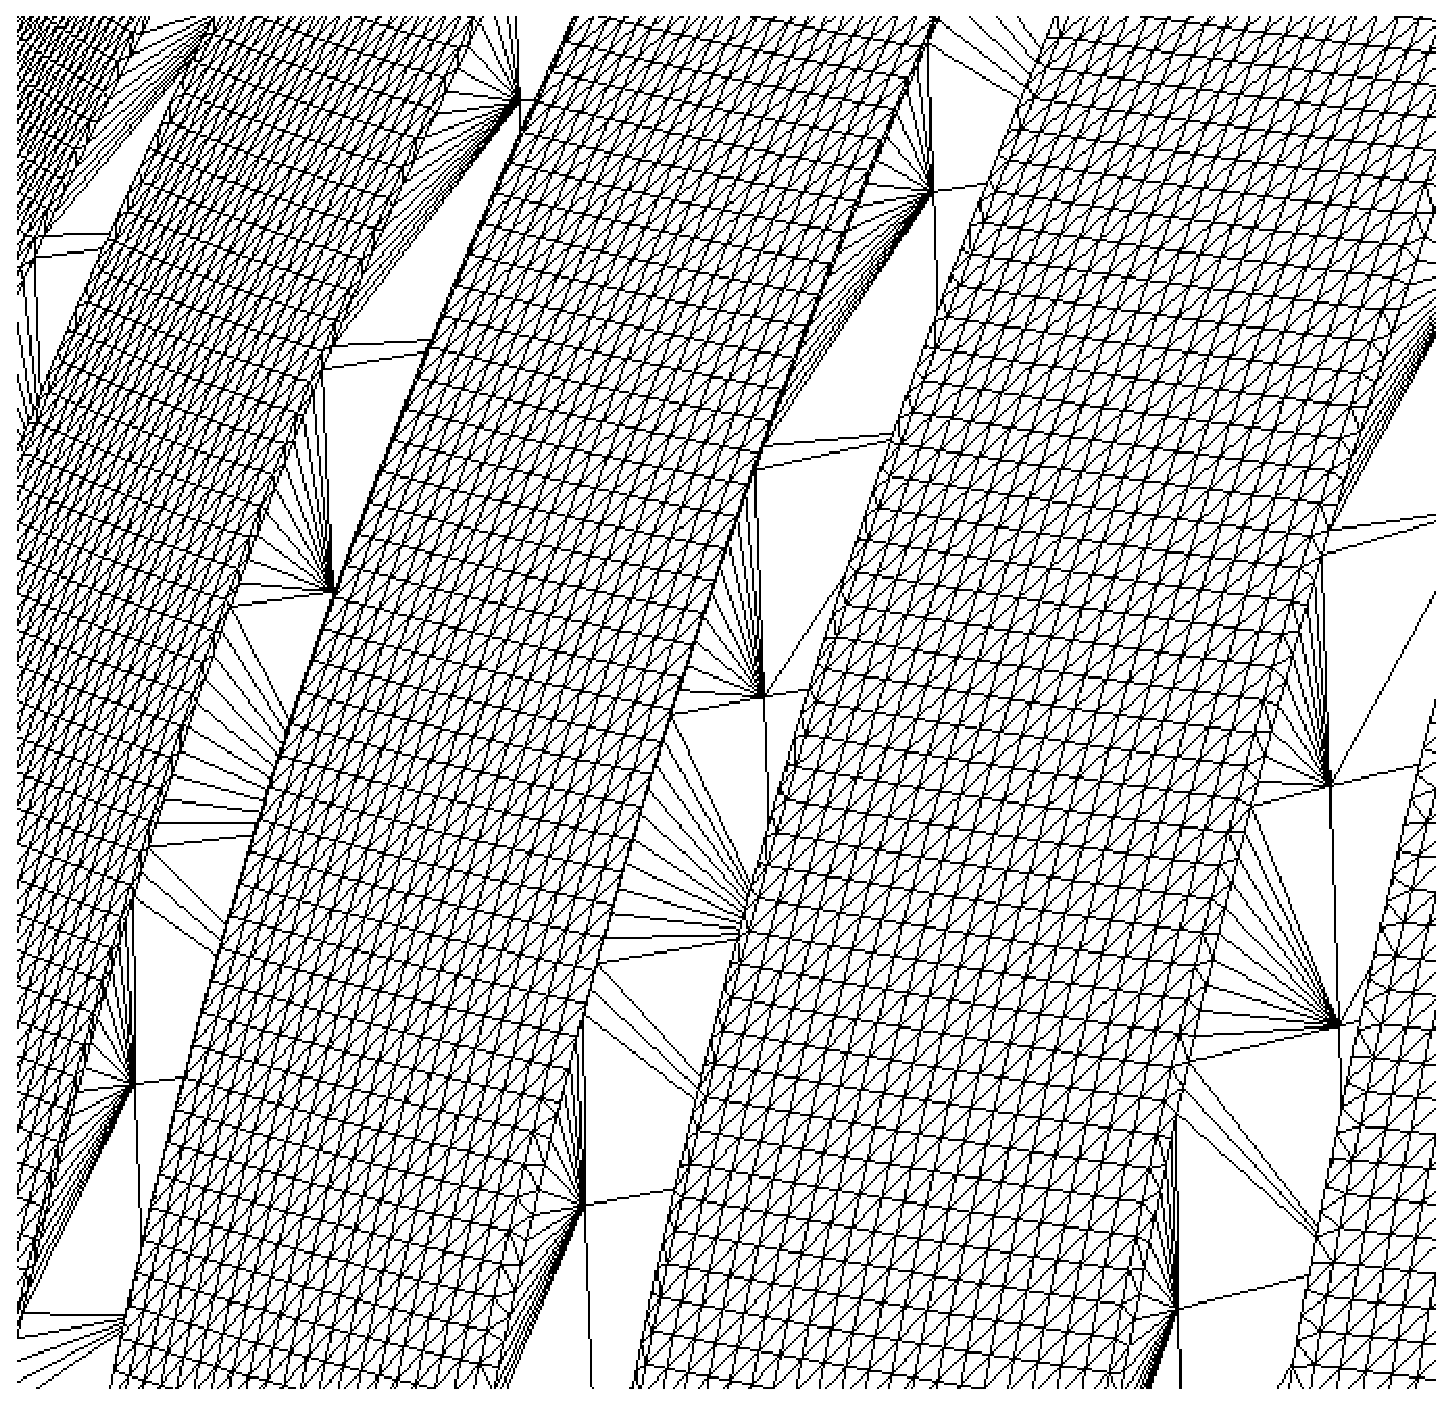
\includegraphics[scale=0.2]{ds_hv.eps}
  \caption{Examples of high valence vertices in analysis and test models.}
  \label{fig:hv_examples}
\end{figure}

These regions are commonly generated in the faceting algorithms used to produce
DAGMC meshes. This faceting scheme (which comes from ACIS libraries underlying
the CUBIT/Trelis graphics engine) is designed to produce the smallest number of
triangles possible to represent the model within the representation tolerance
specified in DAGMC's surface mesh generation preprocessing. This restriction is
favorable to the rasterization process commonly used to display models
interactively in the CAD program. Fewer triangles are better for the purpose
particle tracking in DAGMC as well as long as the geometry is accurately
represented. Even the ideal ray tracing acceleration structure queries for a
given triangle mesh scale as $O(log(N))$, and the size of models being analyzed
using the toolkit provides motivation to keep memory footprints as low as
possible. However, even with fewer triangles undesirable configurations can
impede performance as is shown by a set of tests conducted on models generated
by this faceting scheme.

\section{Previous Work}

A study conducted by Steve Jackson in 2010 on the performance of the MOAB ray
tracer revealed a steep degredation in performance with a decreasing faceting
tolerance or an increasing number of triangles. Using a DAGMC-based ray fire
test program, the performance of DAGMC's ray fire ability was evaluated for four
models. These models include a simple sphere, a notched or slotted sphere, and
an outer volume of an ITER model, shown in Figure \ref{fig:sj_hv_test_models}.

\begin{figure}[H]
    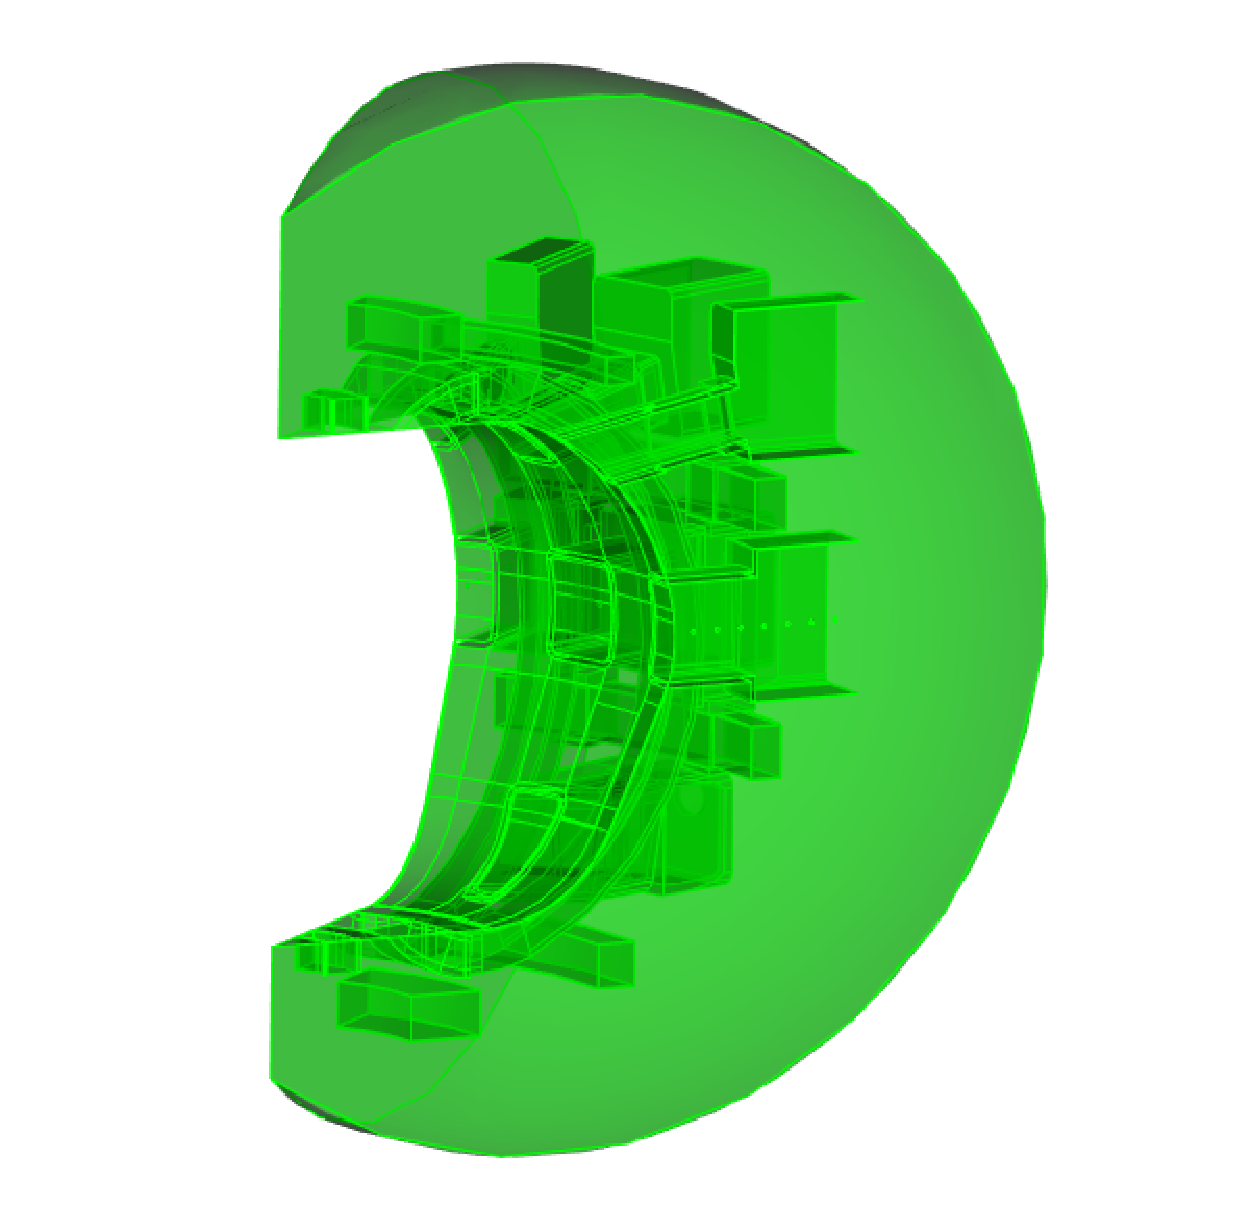
\includegraphics[scale=0.32]{iter_rf_vol.eps}
    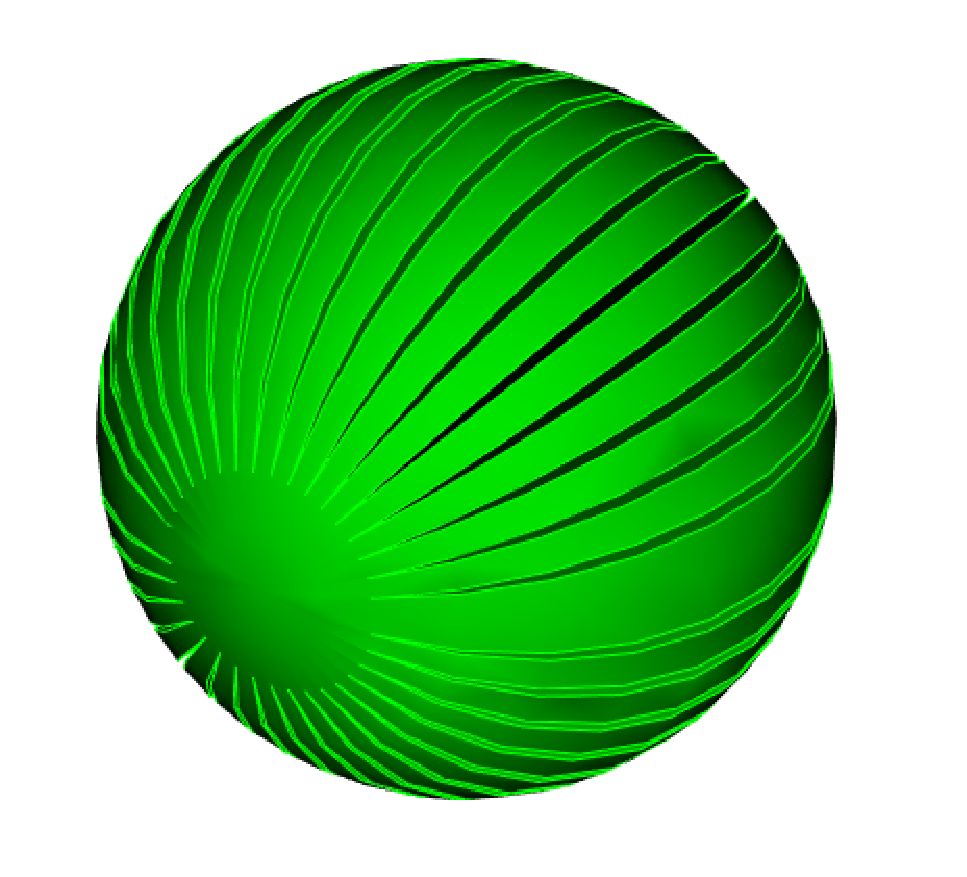
\includegraphics[scale=0.42]{ds.eps}
\begin{center}
  \caption{Images of the slotted sphere and ITER volume used to perform DAGMC
    ray fire performance tests with increasing number of triangles or,
    equivalently, decreasing faceting tolerance.}
\end{center}
\label{fig:sj_hv_test_models}
\end{figure} 

In each of these tests, the models are tesselated with an increasingly smaller
faceting tolerance where the faceting tolerance being defined as the maximum
distance between the faceted curve or surface and the geometric curve or surface
it resolves.  By this definition, the number of triangles needed to represent a
model is inversely proportional to the value of the faceting tolerance. An
increase in the number of triangles leads to a more complex nature of the
surface mesh in terms of BVH construction and traversal.

Each model used in these tests presents its own challenges with increasing
faceting tolerance. The sphere is a good control case for an increasing number
of triangles without change in complexity or exacerbation of pathological mesh
features. The number of triangles generated in the spherical case will tend
toward a maximum value with decreasing faceting tolerance, but the general
nature of the triangulated surface (triangle density, structure, etc.)  will
remain the same. This is not true of geometries with planar surfaces which may
be able to be resolved exactly using some finite number of triangles making the
sphere a vaulable test model in that regard. In the case of the notched sphere,
high-valence regions are generated by the faceting engine as a result of its
underlying algorithms for planar surfaces meeting curves surfaces. The high
triangle density of high valence regions causes overlaps in bounding volumes
which become larger as the faceting tolerance decreases. This results in
inefficient hierarchy traversal. Additionaly, and perhaps more importantly than
the presence of high valence regions, rays being fired with a point of origin at
the center of the model causes them to travel either exactly along or very near
to the surfaces of the planar slots in the sphere. Such a ray query will visit
many internal nodes of the hierarchy during traversal, creating what is referred
to as a very wide traversal through the BVH as opposed to a narrow traversal in
which fewer branches and fewer nodes of the tree are visited. In this way, the
slotted sphere provides a good measure for the performance of a wide traversal
through the hierarchy in a situation for which many of the internal nodes are
required to be visited. Finally, the faceting of a volume from an ITER model is
used as a production demonstration of the effect of high valence regions on
DAGMC performance (see Figure \ref{fig:hv_examples}).

\begin{figure}[H]
  \begin{center}
    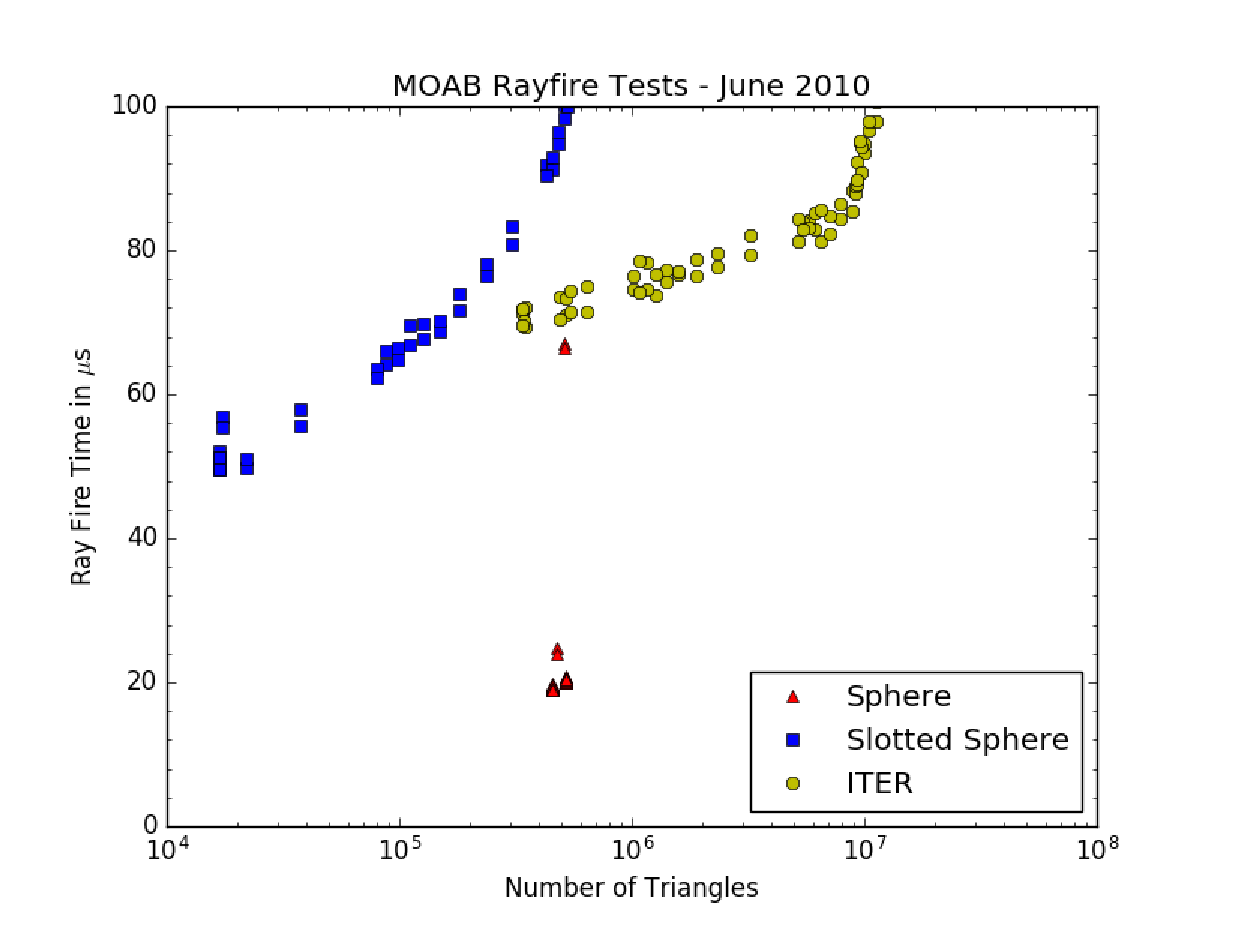
\includegraphics[scale=0.5]{sj_hv_test_results_2010.eps} \\
    \caption{Results of MOAB ray tracing performance tests with decreasing
      faceting tolerance performed by Steve Jackson in June of 2010. Data points
      represent average time spent in firing a ray for random rays
      originating at the center of each model.}
    \label{fig:sj_hv_test_results}
  \end{center}
\end{figure}

While the sphere model shows good scaling with increasing number of triangles,
the ITER volume and slotted sphere both have a pronounced increase in average
ray fire time with decreasing faceting tolerance. Knowing that both of the
latter models contain high valence regions, it was postulated at the time that
these regions had a significant effect on the scaling. 

\section{Characterization and Testing}

In order to isolate the high-valence vertex problem generated by the ACIS
graphics faceting algorithm used in Cubit/Trelis, a test model was manually
generated in MOAB with an artificial high-valence region (shown in Figure
\ref{fig:hv_cube_design}). This mesh is a modified cube mesh centered on the
origin in which one of the two-triangle surfaces has been replaced by a more
complex planar surfce of triangles including an interior high-valence region
within the face. The high-valence region was generated by inserting vertices
along the diagonal of the interior box and connecting them to the opposing
corners of the box. This mesh is generated using two parameters: the valence of
the corner vertices in the interior region and the relative size of the interior
region. Tests were then peformed by varing these two parameters in order to
characterize the performance impediment and determine its root cause.

\begin{figure}[H]
  \centering
    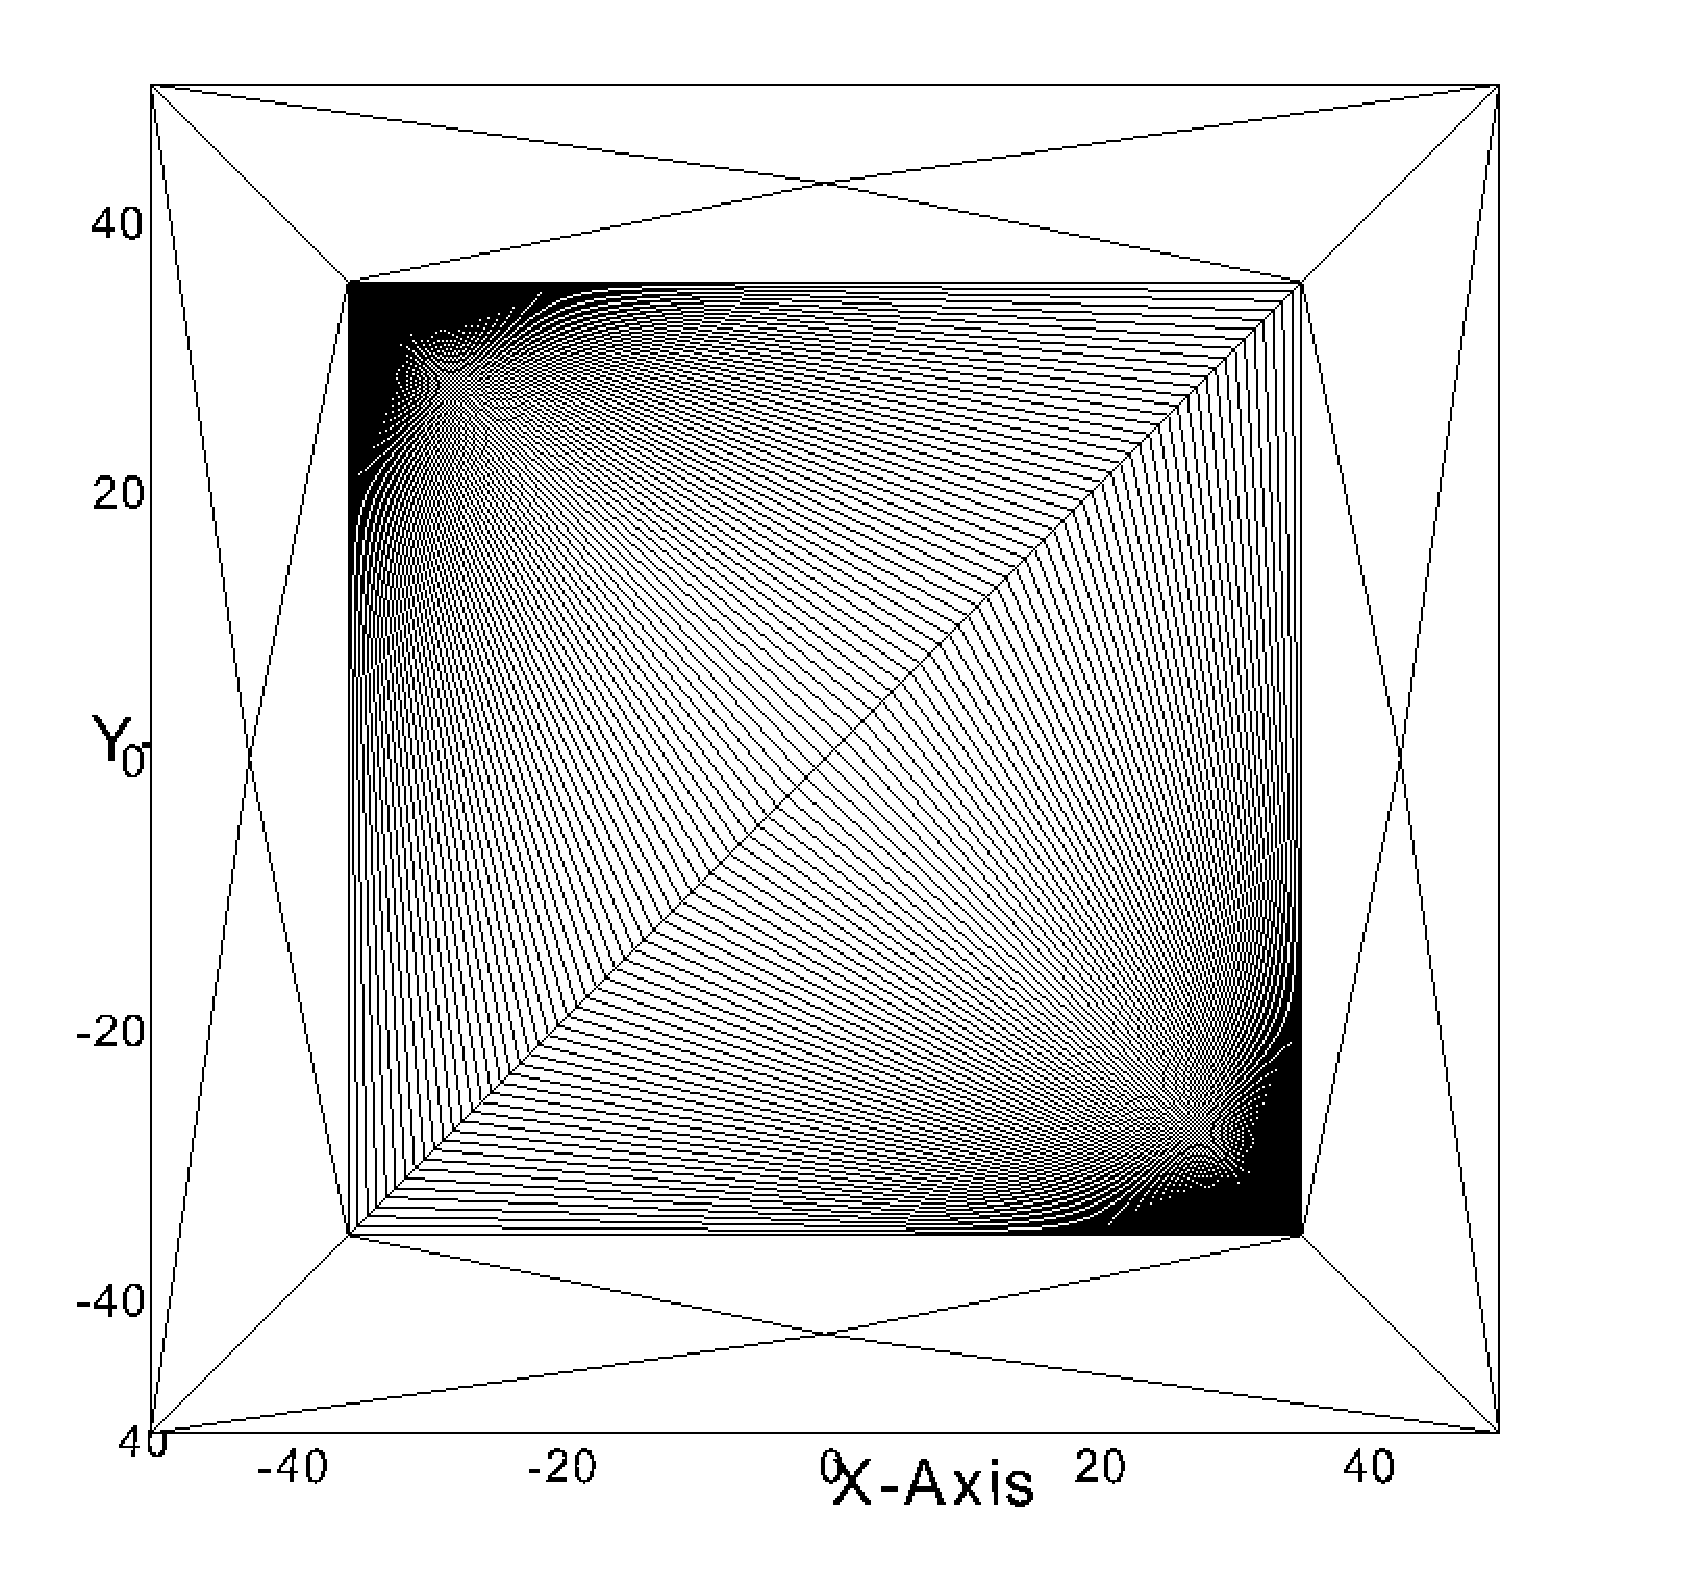
\includegraphics[scale=0.33]{hv_study_design.eps}
    \caption{Side-on view of the modified cube mesh used to study the
      high-valence vertex problem.}
    \label{fig:hv_cube_design}
\end{figure}

A ray fire test program was used to construct MOAB's BVH and perform ray queries
using DAGMC's interface. Information on this test program can be found in the
appendix of this work. This program was used to fire rays with random direction
from the origin of the high valence test model while biasing the ray directions
such that they should always find intersections on the modified surface
containing the high-valence region. A parameter sweep was performed by varying
the percentage of the surface covered by the high-valence region as well as the
valence of the region. Specification of the random number seed is allowed within
the program to giving a more direct comparison of performance with the guarantee
that the same set of rays is fired in each test case. Each test shown in this
section varies the valence of the corner vertices from 2 to 50,000 and the
relative area of the high valence region from 0 to 1.

\section{MOAB's Oriented Bounding Box Tree}\label{sec:hv_study_MOAB}

From what is known about the construction of MOAB's BVH, it was expected that
the average ray fire time would be most strongly correlated to the relative area
of the high valence region, but would also increase with increasing valence of
the corner vertices. The initial results of this study, shown in Figure
\ref{fig:hv_study_moab}, meet only one of the expectations however. The ray fire
times become far worse with increase in valence, but for a constant valence, the
smaller relative area models show a longer average ray fire time than the models
with larger relative areas. This suggests that the presence of a high-valence
region in a surface is detrimental to performance regardless of the likely hood
that a ray intersects with a triangle in that region. In order to investigate
this matter further, a visualization tool for MOAB's BVH was developed to
improve the author's intuition about this mesh pathology.

\begin{figure}[H]
  \centering
    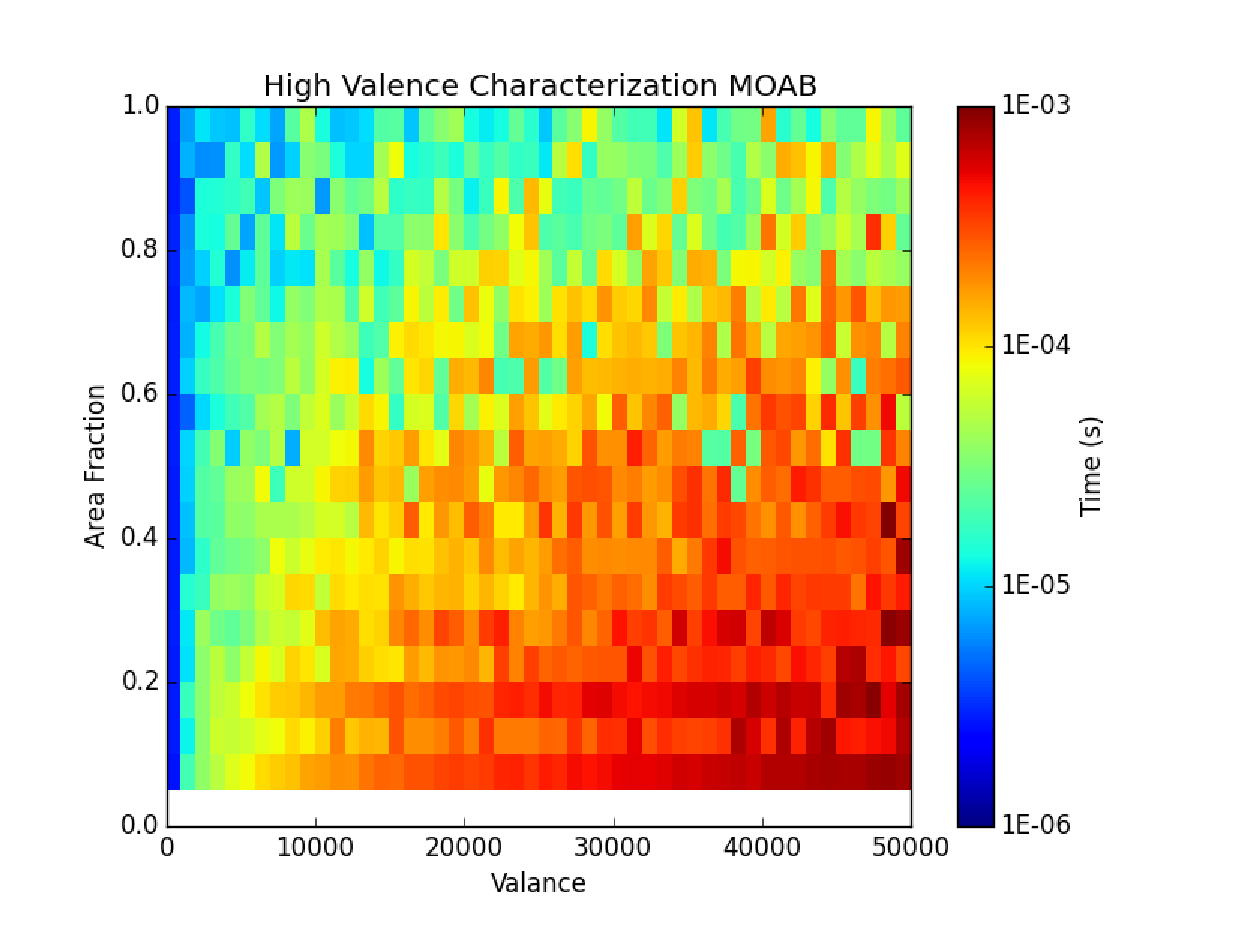
\includegraphics[scale=0.55]{hv_study_MOAB.eps}
    \caption{Results from parameter sweep of valence and valence area fraction
      in the high-valence test mesh.}
    \label{fig:hv_study_moab}
\end{figure}


\subsubsection{Visualization and Diagnosis}\label{subsec:hv_vis}

Using the same visitor pattern employed to traverse rays through the hierarchy,
each OBB in the HV model tree was converted into a hex element and saved in a
VTK mesh format. Each hex element representing an OBB was tagged with its
depth in the tree as well as the triangle entities it contains, if any. These
mesh files can then be used to visualize the hierarchy level-by-level
superimposed on the geometric mesh. An example of this OBB visualization for the
high valence characterization model is shown in Figure \ref{fig:bad_hv_box}. 

\begin{figure}[H]
  \centering
    \includegraphics[scale=0.3]{{obbs_wsr_0.95}.eps}
    \caption{View of culprit bounding box containing many high valence region
      triangle as well as other surface triangles. Blue box and triangles: leaf
      node bounding box and associated triangles. Several thousand
      triangles are represented in the solid blue region shown here. Red boxes: Other
      representative boxes at the same depth in that tree.}
    \label{fig:bad_hv_box}
\end{figure}

Because there are more entities to partition in the high valence region, it is
expected the lowest levels of the BVH will contain only OBB's bounding triangles
in that region. It was expected that leaf nodes of the BVH might contain many
triangles of the high valence region, causing performance degradation of ray
traversal in that many triangles must be checked for intersection. These types
of poorly formed leaf nodes shift the complexity of the traversal back toward a
linear search - which is sub-optimal. This feature of the produced BVH's in MOAB
were observed, but visualization of the BVH provided the ability to observe
another characteristic as well. Many leaf nodes containing large numbers of
triangles in the high valence region also contained one or two large triangles
outside of that region. The inclusion of these large triangles significantly
increases the probability that a hierarchy traversal will visit that leaf node
and thus all of the triangles contained by that leaf node. This artificial
increase in the high valence regions cross-section greatly exacerbates the
already poorly created nodes in the tree.

Due to the nature of the entity ratio heuristic used to divide nodes in the
tree, as the high valence region becomes smaller more triangle centroids are
shifted onto one side of the median splitting planes used to divide the nodes
which contain portions of that region. If enough triangle centroids are on this
side of the plane, then the cost of the entity ratio evaluation will exceed the
preset upper limit of the cost (0.95 in MOAB) and the construction process will
declare that node a leaf node. This settings governing this split process can be
altered in MOAB, and changing the worst split ratio to 1.0 significantly
improves the average ray fire time in the high valence characterization study,
as seen in Figure \ref{fig:hv_study_moab_wsr1}.

\begin{figure}[H]
  \centering
    \includegraphics[scale=0.55]{{hv_study_MOAB_wsr1}.eps}
    \caption{Results of the high valence characterization study with a worst
      case splitting ratio set to 1.}
    \label{fig:hv_study_moab_wsr1}
\end{figure}

As expected, the use of this setting largely removes the degradation in performance
caused by the high valence region by forcing the continued splitting of entities
in the tree where large leaf nodes would have been created before. This
demonstrates that altering this setting works well for this mesh feature, but it
would be detrimental to the memory footprint of the overall hierarchy in the
general case, causing certain areas of the tree to be over-refined. 


\subsection{Adaptive BVH Construction}\label{subsec:adaptive_construction}

One of the benefits to having a BVH tool which is part of a mesh database like
MOAB is the ability to query for more information about the mesh when
constructing hierarchies like the BVH. This information has been used to detect
high valence regions in the mesh and adapt BVH construction to improve the
hierarchy quality in these areas.

\subsubsection{High Valence Detection}\label{subsubsec:hv_detection}

A simple algorithm is used to determine whether or not the entities inside a
leaf node are part of a high valence region. Any vertex connected to more than
$\alpha$\% of the entities in a given leaf node will be considered a high valence
region, indicating that an alternate build method or build settings should be
applied.

\begin{lstlisting}
  def detect_hv_region(mesh, entities, alpha):
      assert(a <= 1.0 and a > 0.0)
      connectivity = mesh.get_connectivity(entities)

      to_dim = 2
      for vertex in connectivity:
          # get all entities of dim 2 adjacent to the vertex
          adj_entities = mesh.get_adjacencies(vert, to_dim)

          # determine how many adj entities are in the set of entities
          overlap = entities - adj_entities

          if( size(overlap)/size(entities) < 1.0 - alpha):
              return true

      return false
\end{lstlisting}

\subsubsection{Implementation}\label{subsec:adaptive_construction_implementation}

First, MOAB's BVH constructor was modified with the option of tagging poorly
formed leaf nodes in the tree. This option will apply a tag to any leaf nodes
which contain more entities the specified in the settings for the tree. These
nodes are then revisited for further refinement later in the build process.

For handling of these poorly formed leaf nodes, a new class was created in MOAB
named the \textit{BVHRefiner}. This class visits each leaf node tagged by the
build process to determine if further refinement is appropriate based on the
available set of mesh features it is capable of handling. For each mesh feature
added to the BVH Refine class, a detection method and build method is
required. This class applies these detection methods and altered build methods
to resolve these leaf nodes into improved regions of the tree. The intent of
this design was to support the detection and adaptation to other pathological mesh
features.

In the high valence case, the refiner class will search for any vertex connected
to more than 80\% of the entities in that particular leaf node. If this condition
is met, the leaf node is declared part of a high valence region and an altered
build method is applied. For the HV case, this build method has been established
by previous work as the standard build algorithm with the worst case splitting
ratio set to 1.0.

\subsubsection{Application to the HV test model}

This adaptive build method was applied to the high valence test model as
before. The results of this test can be seen in Figure
\ref{fig:hv_study_adaptive}. Using the adaptive method, the average ray fire
time is consistent across both valence and relative area of the HV region.

\begin{figure}
  \centering
  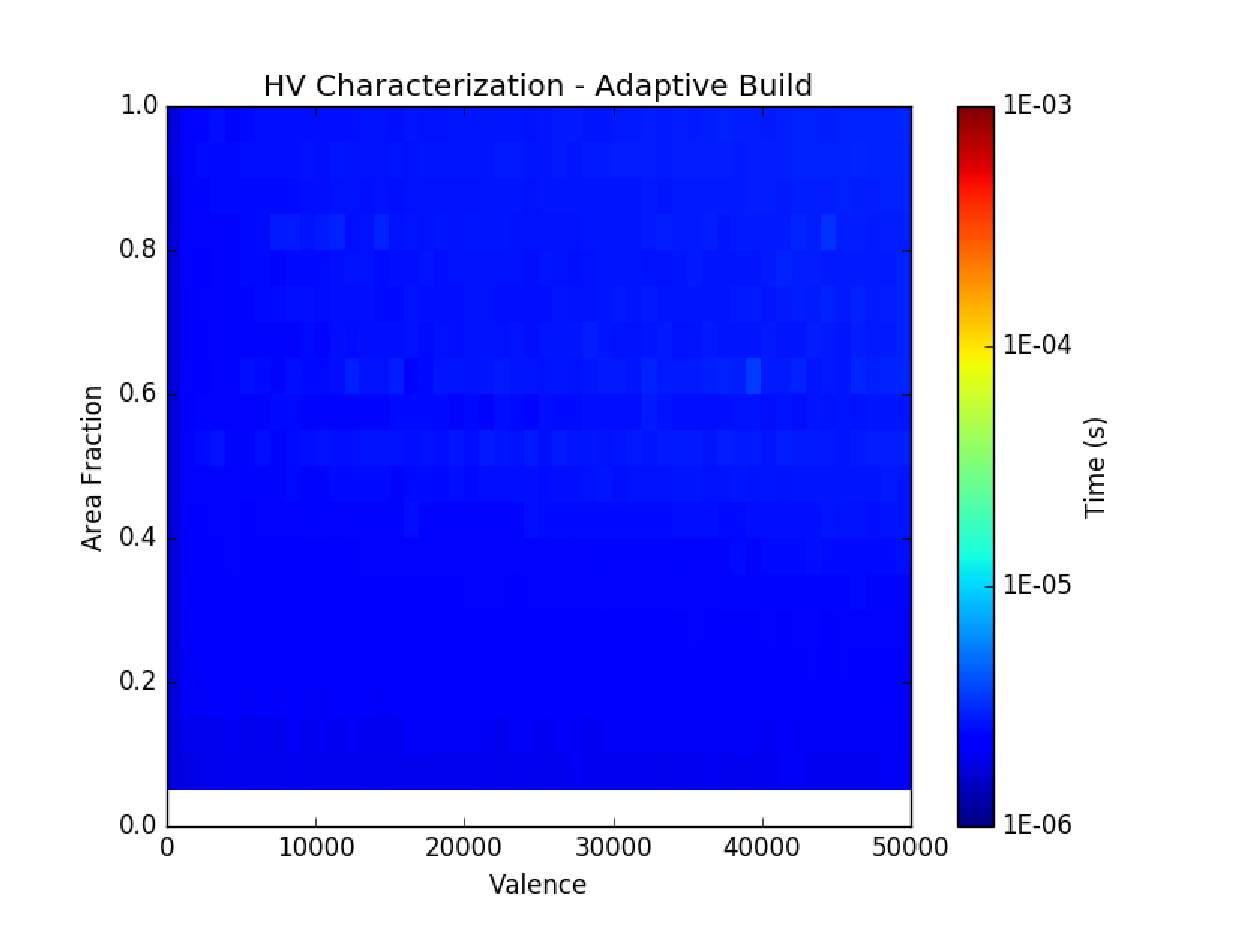
\includegraphics[scale=0.55]{hv_study_moab_adaptive.eps}
  \caption{High valence characterization study with the adaptive BVH building method
    applied.}
  \label{fig:hv_study_adaptive}
\end{figure}

\subsubsection{Application in Production}

This method was also applied to several DAGMC production models in order to determine
its effect on simulation runtimes during transport.

\begin{table}[H]
  \centering
  \begin{tabular}{c c c c c}
    \toprule
    \textbf{Model} & \textbf{HV Regions} & \textbf{Particle Histories} & \textbf{Runtime reduction} & \textbf{Buildtime increase} \\
    \hline
    FNG            & 514                 & 1M                          & 3.3\%                      & 18.5\%                      \\
    ITER-BLITE     & 3522                & 1M                          & 23.4\%                     & 5.2\%                       \\
    \bottomrule
  \end{tabular}
  \caption{Results of runtime reduction in several DAGMC production models when applying the BVH refinement.}
  \label{tab:bvhrefine_production_results}
\end{table}    

In the case of FNG, the runtime is decreased only marginally, but in the ITER
model the runtime is reduced by nearly $\frac{1}{4}$. It can be presumed that
the reduction in the runtime is associated with the frequency with which a HV
nodes in MOAB's OBB tree are visited. In the FNG model, the HV regions tend to
be smaller and adjacent to the graveyard of the problem while in ITER there are
large HV regions occupying large portions of the external reflecting surfaces of
the model. This provides some anecdotal information about why the refinement has
a larger effect in the ITER model than in the FNG model. It is possible,
however, to quantify this effect more thoroughly by counting the number of HV
node visits in either case during simulation.

\section{Embree's Ray Tracing Kernel}\label{sec:emdag_hv_study}

The same test described in Section \ref{sec:hv_study_MOAB} was performed
using the ray fire test program compile with using EmDAG to fire rays. A
different behavior was expected when using Embree to construct the underlying
hierarchies due to its use of the SAH. Figure \ref{fig:hv_study_emdag} contains
the results of this test run. Using the Embree kernel, the performance degrades
in direct proportion to both valence and the relative area of the high valence
region. This data represents the expected behavior of MOAB's BVH. Unlike MOAB
however, Embree's use of the surface area heuristic prevents the artificial
increase in probability of visiting triangles in the high valence region. Larger
triangles adjacent to this region are more readily separated from the leaf due
to the additional cost they add by increasing a bounding box's surface area and
in turn its evaluated cost. Separation of triangles in the HV region itself is
still difficult when restricted to axis-aligned candidate split planes.

\begin{figure}[H]
  \centering
    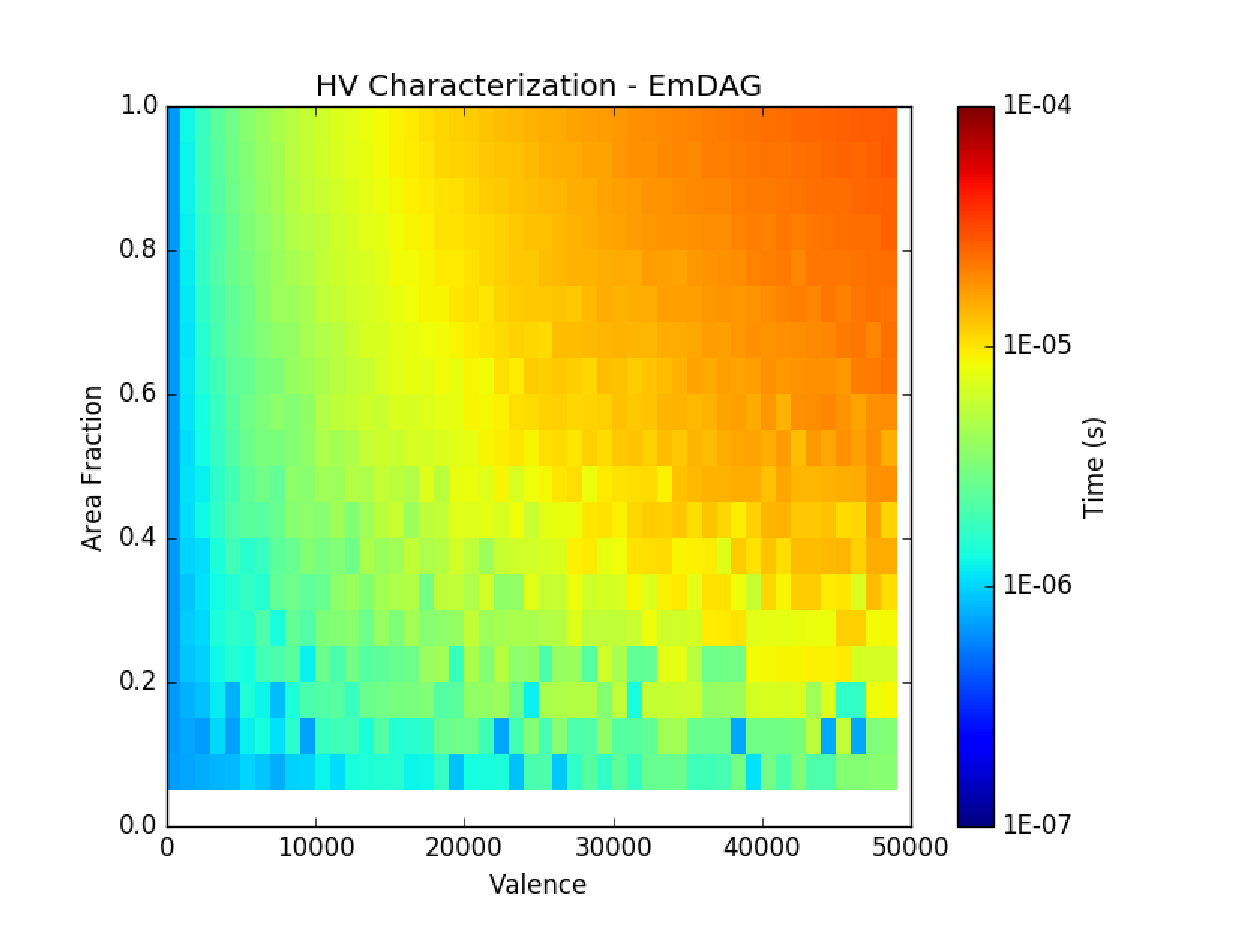
\includegraphics[scale=0.55]{hv_study_emdag.eps}
    \caption{High valence parameter study results when applying Intel's Embree
      within the DagMC ray fire program.}
    \label{fig:hv_study_emdag}
\end{figure}

While this data provides evidence that HV regions are problematic for
production-level ray tracing kernels, it is difficult to employ any adaptive
tree construction techniques. Without access to the underlying mesh
representation of the triangle surface, it is difficult to detect HV regions as
implemented in MOAB's OBBTree. This is both a strength and weakness of Embree's
design in that it can build highly efficient datastructures using only primitive
point and connectivity data, but it has no infrastructure in place to
interrogate that data deeply. Methods for detecting and adapting to these HV
regions are addressed using the MMPBVH, a system with similar characteristics
but with more access to the mesh interface.

\section{Mixed Precision Bounding Volume Hierarchy}\label{sec:simd_hv_study}

The MPBVH kernel created by the author has a similar trend to Embree's
kernel where ray fire times increase proportionally to both the valence and size
of the high valence region. The author's BVH applies a modified form of the
surface area heuristic in which the surface area of the box is weighted by the
number of entities it contains to determine if a split is beneficial or
not. Near HV regions this heuristic is able to separate large triangles from the
HV region in the same way as the unmodified surface area heuristic, but it
fails to create a well-structured tree for triangles that are part of the HV area.

\begin{figure}[H]
  \centering
    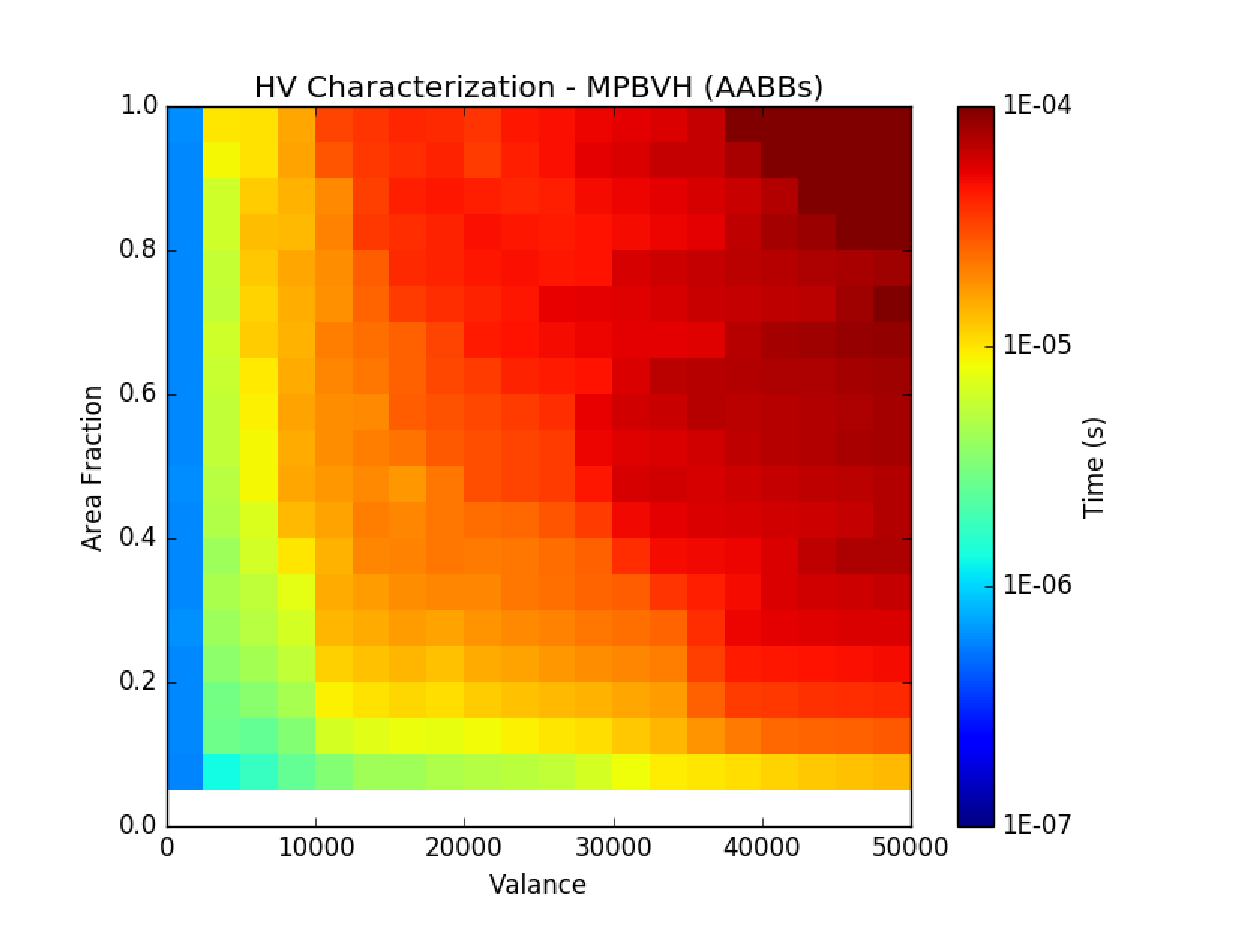
\includegraphics[scale=0.55]{hv_study_SIMD.eps}
    \caption{High valence parameter study results for the MPBVH kernel.}
    \label{fig:hv_study_simd}
\end{figure}

\subsection{Visualization and Diagnosis}

Visualization of leaf nodes and the entities they contain for the MOAB SIMD BVH
can be seen in Figure \ref{fig:hv_leaf_simd_bvh}.

  \begin{figure}
    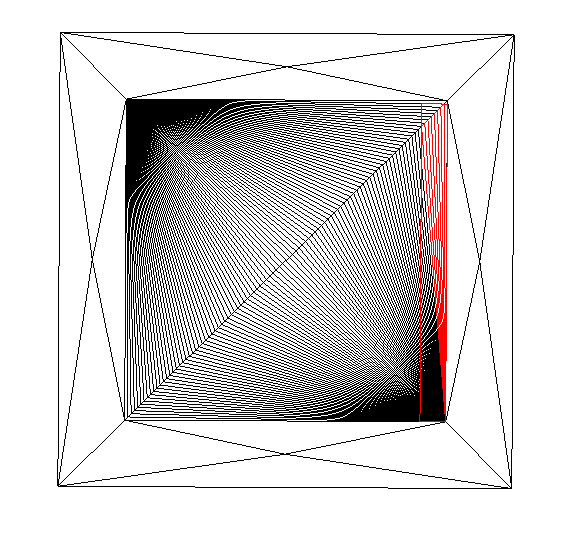
\includegraphics[scale=0.5]{hv_leaf_simd_bvh.png}
    \caption{MOAB SIMD BVH leaf nodes for the HV test model with area fraction
      0.5 and a valence of 100 for the corner vertices.}
    \label{fig:hv_leaf_simd_bvh}
  \end{figure}
  
Both Embree and the MOAB SIMD BVH have the shared characteristic of a limited
leaf size of eight primitives due to the way the leaves are encoded. This
removes the possibility that large numbers of triangles in leaf nodes as the
cause of performance degradation, which was true for MOAB's OBB Tree. In the case
of Embree and the MBVH, the largest cause of performance degradation is
overlapping regions of the leaf nodes.

Because both of these implementations use AABBs, bounding of skinny, off-axis
triangles results in bounding boxes with a considerable amount of empty space in
them. An example of such a leaf can be seen in Figure
\ref{fig:hv_overlap_simd_bvh}. In high valence regions, this results in the same
space being occupied by a high number of leaf bounding boxes. If a ray is fired
into these overlapping leaves, the end result is a large number of leaf nodes,
and in turn, triangles, visited.

\begin{figure}
  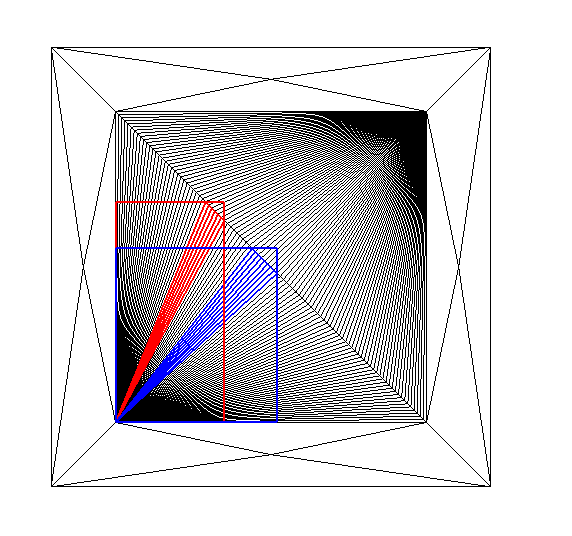
\includegraphics[scale=0.5]{hv_overlap_simd_bvh.png}
  \caption{Visualization of a large bounding box surrounding low aspect ratio,
    off-axis triangles.}
  \label{fig:hv_overlap_simd_bvh}
\end{figure}

To alleviate the effect of the overlapping AABBs in this region, OBBs were
implemented as part of the MPBVH. Figure \ref{fig:hv_study_simd_obbs} shows the
results of this study. Because the simplified SAH heuristic is able to separate
large triangles exterior to the HV region into different leaf nodes and the
maximum leaf node size is predetermined, scaling very similar to the MOAB OBB
implementation after HV refinement is applied can be seen, though the overall
speed is somewhat improved due to the single precision implementation.

\begin{figure}
  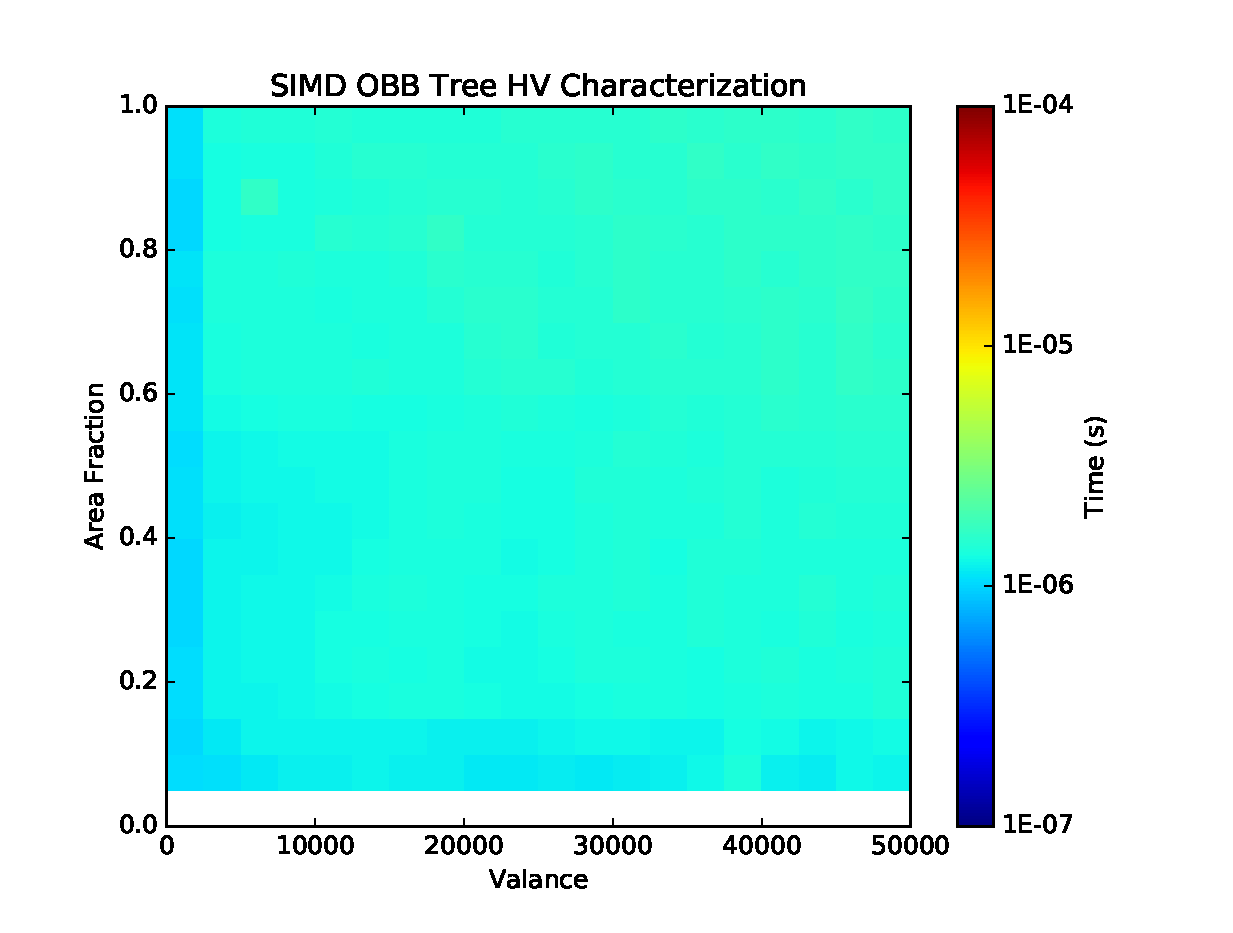
\includegraphics[scale=0.55]{hv_study_SIMD_OBB.eps}
  \caption{High valence vertex study for the MOAB SIMD kernel using OBBs.}
  \label{fig:hv_study_simd_obbs}
\end{figure}

\subsection{Adaptive Construction: Mixed AABB/OBBs}

The solution to HV regions when using the SIMD BVH kernel proposed by the author
is to apply OBBs only in regions determined to be high valence using the same
detection method described in Section \ref{subsubsec:hv_dectetion}. Large leaf
nodes being split into smaller nodes will apply oriented bounding boxes to
contain entities if the set of triangles is determined to be a high valence
region using the same method discussed in Section \ref{subsec:hv_detection}.

\subsubsection{Additional Node Encoding}

To support a tree containing both AABBs and OBBs, additional encoding of
interior nodes is required so that the appropriate node intersection methods are
applied during traversal. The additional encoding representation for these node
types can be seen in Figure \ref{fig:mixed_node_encoding}. This encoding scheme
takes advantage of the two remaining bit configurations availble for node
definitions by setting the appropriate bits in the node reference objects. These
node masks are stripped from the node reference's integer value to retrieve the
pointer to the node objects themselves with little added overhead in the
traversal process.

\begin{figure}[H]
  \includesvg{../images/mixed_node_encoding}{1.0\textwidth}
  \label{fig:mixed_node_encoding}
\end{figure}

\subsubsection{OBB Implementation}

The same covariance method used in MOAB to construct OBB's was applied in the
MPBVH, but the storage technique used differs in order to accomodate the SIMD
programming involved in the BVH traversal. OBB nodes are stored as scaled,
affine transformations of the global problem space and the box's lower left
corner is stored as a scaled reference point. When a ray is intersected
with a node it is transformed and scaled at the same time, but separately, for
each of the four OBBs the node represents. A recipricol direction is then
calculated with respect to the oriented axes of each box. Intersection values
and distances are then returned in the same way they are calculated for a node
of AABBs.

OBB nodes contain additional information in the form of the affine space
transformation and are more computationally expensive when computing ray
transformations. Some of this computational cost is avoided by incorporating the
spatial scaling of the node into both the affine space and reference point to
avoid the additional computational cost of scaling the parametric values of the
ray intersection later in the calculation.


